\documentclass[11pt,letterpaper]{article}
\usepackage[margin=1in]{geometry}
\usepackage{graphicx}
\usepackage{amsmath,amssymb}
\usepackage{booktabs}
\usepackage{float}
\usepackage{hyperref}
\usepackage{xcolor}
\usepackage{caption}
\usepackage{subcaption}
\usepackage{enumitem}
\usepackage{fancyhdr}

\pagestyle{fancy}
\fancyhf{}
\rhead{RAMP Algorithm Technical Report}
\lhead{Rubin Observatory}
\rfoot{Page \thepage}

\title{\textbf{RAMP: Rubin Anticipatory Mirror Protocol}\\[0.5em]
\Large A Three-Phase Thermal Control Algorithm for\\Primary Mirror Temperature Management}

\author{Rubin Observatory Thermal Control Study\\[0.5em]
\small January 2026}

\date{}

\begin{document}

\maketitle

\begin{abstract}
This report describes the development and optimization of the \textbf{RAMP} (Rubin Anticipatory Mirror Protocol) algorithm for thermal control of the Rubin Observatory primary mirror. The goal is to maintain the mirror temperature at 0.3$^\circ$C below ambient to minimize thermal turbulence during nighttime observations. We evaluate multiple control strategies including reactive, predictive, and hybrid approaches, and present a three-phase control system optimized through grid search over $\sim$770 nights of historical temperature data. The optimal RAMP configuration achieves overnight RMS errors of $\sim$0.20$^\circ$C with $>$90\% of observations within the $\pm$0.3$^\circ$C target band.
\end{abstract}

\tableofcontents
\newpage

%==============================================================================
\section{Introduction and Problem Statement}
%==============================================================================

\subsection{Background}

The Vera C. Rubin Observatory, located at Cerro Pach\'{o}n, Chile (latitude $-30.2444^\circ$, longitude $-70.7494^\circ$), requires precise thermal management of its primary mirror to achieve optimal image quality. Temperature differences between the mirror surface and ambient air create convective turbulence directly above the optical surface, degrading image quality through a phenomenon known as ``mirror seeing.''

\subsection{Control Objective}

The thermal control system must maintain the mirror temperature at a \textbf{cold bias} of 0.3$^\circ$C below ambient:
\begin{equation}
T_{\text{target}}(t) = T_{\text{ambient}}(t) - 0.3\,^\circ\text{C}
\label{eq:target}
\end{equation}

This slight cooling prevents warm air from rising off the mirror surface while avoiding condensation risks associated with excessive cooling.

\subsection{Operating Constraints}

The thermal control system operates under the following physical constraints:

\begin{itemize}[noitemsep]
    \item \textbf{Mirror thermal time constant}: $\tau = 2$ hours
    \item \textbf{Maximum HVAC setpoint change rate}: $\pm 2\,^\circ$C/hour
    \item \textbf{Daytime operation}: Dome closed, mirror temperature controlled by HVAC
    \item \textbf{Nighttime operation}: Dome open, mirror exposed to ambient conditions
\end{itemize}

The 2-hour thermal time constant means the mirror cannot respond instantaneously to setpoint changes, requiring anticipatory control strategies.

%==============================================================================
\section{Physical Model}
%==============================================================================

\subsection{Thermal Dynamics}

The mirror temperature evolution follows first-order dynamics:
\begin{equation}
\frac{dT_{\text{mirror}}}{dt} = \frac{T_{\text{setpoint}} - T_{\text{mirror}}}{\tau}
\label{eq:dynamics}
\end{equation}

where $\tau = 2$ hours is the thermal time constant. This differential equation has the solution:
\begin{equation}
T_{\text{mirror}}(t) = T_{\text{mirror}}(0)\,e^{-t/\tau} + \frac{1}{\tau}\int_0^t T_{\text{setpoint}}(s)\,e^{-(t-s)/\tau}\,ds
\end{equation}

\subsection{Theoretical Optimal Control}

For perfect tracking of a time-varying target, control theory indicates the setpoint should anticipate the target by the time constant $\tau$:
\begin{equation}
T_{\text{setpoint}}(t) = T_{\text{target}}(t + \tau) = T_{\text{ambient}}(t + \tau) - 0.3\,^\circ\text{C}
\label{eq:optimal}
\end{equation}

This requires perfect prediction of ambient temperature $\tau$ hours into the future. The RAMP algorithm implements practical approximations to this theoretical optimum.

%==============================================================================
\section{Control Algorithm Options Assessed}
%==============================================================================

We evaluated a comprehensive suite of control algorithms spanning reactive, predictive, and hybrid approaches.

\subsection{Baseline Algorithms}

\begin{table}[H]
\centering
\caption{Baseline control algorithms}
\begin{tabular}{lp{8cm}}
\toprule
\textbf{Algorithm} & \textbf{Description} \\
\midrule
Naive & $T_{\text{sp}} = T_{\text{amb}} - 0.3$ (no anticipation) \\
Reactive (rate-based) & $T_{\text{sp}} = T_{\text{amb}} + \tau \cdot \dot{T} - 0.3$ \\
\bottomrule
\end{tabular}
\end{table}

\subsection{Lookahead Algorithms}

These algorithms use predicted future temperatures (assuming perfect prediction capability):

\begin{table}[H]
\centering
\caption{Lookahead control algorithms}
\begin{tabular}{lp{8cm}}
\toprule
\textbf{Algorithm} & \textbf{Description} \\
\midrule
Lookahead $\tau/2$ (1h) & $T_{\text{sp}} = T_{\text{amb}}(t+1) - 0.3$ \\
Lookahead $\tau$ (2h) & $T_{\text{sp}} = T_{\text{amb}}(t+2) - 0.3$ \\
Lookahead $1.5\tau$ (3h) & $T_{\text{sp}} = T_{\text{amb}}(t+3) - 0.3$ \\
Lookahead + rate & $T_{\text{sp}} = T_{\text{amb}}(t+\tau) + \tau \cdot \dot{T}(t+\tau) - 0.3$ \\
\bottomrule
\end{tabular}
\end{table}

\subsection{Blended Algorithms}

Weighted combinations of reactive and predictive components:
\begin{equation}
T_{\text{sp}} = w_{\text{react}} \cdot \left(T_{\text{amb}} + \tau \cdot \dot{T}\right) + w_{\text{pred}} \cdot T_{\text{amb}}(t+\tau) - 0.3
\end{equation}
where $w_{\text{react}} + w_{\text{pred}} = 1$.

\subsection{Weighted Lookahead Algorithms}

Instead of using a single future time point, these algorithms integrate over a weighted prediction horizon:
\begin{equation}
T_{\text{sp}}(t) = \int_0^{T_{\max}} w(s) \cdot T_{\text{amb}}(t+s)\,ds - 0.3
\label{eq:weighted}
\end{equation}

We tested multiple kernel shapes $w(s)$:

\begin{table}[H]
\centering
\caption{Weighting kernel options}
\begin{tabular}{ll}
\toprule
\textbf{Kernel Type} & \textbf{Functional Form} \\
\midrule
Uniform & $w(s) = 1/T_{\max}$ for $s \in [0, T_{\max}]$ \\
Linear decay & $w(s) \propto (T_{\max} - s)$ \\
Exponential & $w(s) \propto e^{-s/\tau_d}$ \\
Gaussian & $w(s) \propto e^{-(s-\mu)^2/(2\sigma^2)}$ \\
Triangle & Peak at specified time, linear decay to both sides \\
\bottomrule
\end{tabular}
\end{table}

\subsection{Weighted Rate Algorithms}

The most sophisticated approach uses weighted integrals of both temperature and rate:
\begin{equation}
T_{\text{sp}}(t) = \sum_i w_T(s_i) \cdot T(t+s_i) + \tau \sum_j w_r(s_j) \cdot \dot{T}(t+s_j) - 0.3
\label{eq:weighted_rate}
\end{equation}

This captures both the predicted temperature trajectory and its curvature.

%==============================================================================
\section{Optimization Process}
%==============================================================================

\subsection{Data and Train/Test Split}

The optimization used historical temperature data from October 2023 through December 2025:
\begin{itemize}[noitemsep]
    \item \textbf{Total valid nights}: $\sim$770
    \item \textbf{Temporal resolution}: 15 minutes
    \item \textbf{Training set}: Even calendar days ($\sim$385 nights)
    \item \textbf{Test set}: Odd calendar days ($\sim$385 nights)
\end{itemize}

\subsection{Performance Metrics}

Algorithms were evaluated using:
\begin{enumerate}[noitemsep]
    \item \textbf{RMS error}: $\sqrt{\langle(T_{\text{mirror}} - T_{\text{target}})^2\rangle}$
    \item \textbf{Percentage within $\pm$0.3$^\circ$C}: Fraction of time the error is within tolerance
    \item \textbf{Sunset error}: Error magnitude at the moment the dome opens
    \item \textbf{Mean bias}: Systematic over/under-temperature tendency
\end{enumerate}

\subsection{Grid Search Optimization}

For the three-phase control system, we performed exhaustive grid search over:
\begin{itemize}[noitemsep]
    \item Phase transition times $T_1$ and $T_2$ (hours before sunset)
    \item Phase 2 algorithm variants (4 options)
    \item Lookahead kernel parameters ($T_{\max}$, decay time, peak position)
    \item Rate compensation weights
\end{itemize}

Total configurations evaluated: $>$500

\subsection{Weighted Lookahead Optimization}

For the overnight tracking phase, we tested:
\begin{itemize}[noitemsep]
    \item 6 temperature kernel types $\times$ 8 rate kernel types = 48 combinations
    \item Multiple parameter variations per kernel type
    \item Total algorithm variants: $>$200
\end{itemize}

%==============================================================================
\section{The Three-Phase RAMP Algorithm}
%==============================================================================

The optimal control strategy divides operation into three distinct phases based on time relative to sunset.

\subsection{Phase 1: Daytime Fixed Setpoint}

\begin{center}
\fbox{\parbox{0.8\textwidth}{
\textbf{Time}: Sunrise to $T_1 = -3$ hours before sunset\\
\textbf{Dome status}: Closed\\
\textbf{Algorithm}: Fixed setpoint at predicted sunset temperature
\begin{equation}
T_{\text{sp}} = T_{\text{sunset,predicted}} - 0.3\,^\circ\text{C}
\end{equation}
}}
\end{center}

During daytime, the dome is closed and the HVAC system maintains the mirror at a fixed temperature based on the predicted sunset ambient temperature. This pre-positions the mirror for the evening transition.

\subsection{Phase 2: Pre-Sunset Transition}

\begin{center}
\fbox{\parbox{0.8\textwidth}{
\textbf{Time}: $T_1 = -3$ hours to $T_2 = 0$ (sunset)\\
\textbf{Dome status}: Closed (preparing to open)\\
\textbf{Algorithm}: Linear ramp from fixed to tracking
\begin{equation}
T_{\text{sp}} = (1-\alpha) \cdot T_{\text{fixed}} + \alpha \cdot T_{\text{tracking}}
\end{equation}
where $\alpha = (t - T_1)/(T_2 - T_1)$ varies from 0 to 1.
}}
\end{center}

The tracking component includes rate compensation:
\begin{equation}
T_{\text{tracking}} = T_{\text{amb}} - 0.3 + 0.5\tau \cdot \dot{T}
\end{equation}

This phase smoothly transitions from the fixed daytime setpoint to active tracking, ensuring the mirror reaches the correct temperature at dome opening.

\subsection{Phase 3: Overnight Weighted Lookahead}

\begin{center}
\fbox{\parbox{0.8\textwidth}{
\textbf{Time}: $T_2 = 0$ (sunset) to sunrise\\
\textbf{Dome status}: Open\\
\textbf{Algorithm}: Linear-weighted lookahead with rate compensation
\begin{equation}
T_{\text{sp}} = \sum_{i} w_i \cdot T(t + \Delta t_i) + 0.5\tau \cdot \dot{T} - 0.3
\end{equation}
}}
\end{center}

The optimal overnight algorithm uses:
\begin{itemize}[noitemsep]
    \item \textbf{Lookahead horizon}: $T_{\max} = 3$ hours
    \item \textbf{Kernel}: Linear decay from $t$ to $t + T_{\max}$
    \item \textbf{Discretization}: 13 points
    \item \textbf{Rate compensation}: $0.5\tau \times$ current rate
\end{itemize}

The linear decay kernel gives highest weight to near-term predictions (more reliable) while still incorporating longer-term forecasts.

%==============================================================================
\section{Parameter Selection}
%==============================================================================

\subsection{Phase Transition Times}

Grid search over transition times yielded:

\begin{table}[H]
\centering
\caption{Phase transition time optimization results}
\begin{tabular}{ccccc}
\toprule
$T_1$ (hours) & $T_2$ (hours) & Sunset RMS & Overnight RMS & Total \\
\midrule
-5 & 0 & 0.220 & 0.182 & 0.402 \\
-4 & 0 & 0.170 & 0.175 & 0.345 \\
\textbf{-3} & \textbf{0} & \textbf{0.165} & \textbf{0.173} & \textbf{0.338} \\
-2 & 0 & 0.200 & 0.174 & 0.374 \\
-4 & -1 & 0.269 & 0.170 & 0.440 \\
\bottomrule
\end{tabular}
\end{table}

The optimal configuration uses $T_1 = -3$ hours (start ramping 3 hours before sunset) and $T_2 = 0$ (begin full tracking at sunset).

\subsection{Phase 2 Algorithm Selection}

Four Phase 2 variants were tested:

\begin{table}[H]
\centering
\caption{Phase 2 algorithm comparison (with $T_1=-3$, $T_2=0$)}
\begin{tabular}{lcc}
\toprule
\textbf{Phase 2 Algorithm} & \textbf{Sunset RMS} & \textbf{Combined Score} \\
\midrule
\textbf{Ramp fixed$\rightarrow$track} & \textbf{0.165} & \textbf{0.338} \\
Track + $0.5\tau \times$rate & 0.223 & 0.404 \\
Lookahead ramp & 0.270 & 0.439 \\
Track + $\tau \times$rate & 0.282 & 0.455 \\
\bottomrule
\end{tabular}
\end{table}

The simple linear ramp from fixed to tracking outperforms more aggressive approaches.

\subsection{Lookahead Kernel Optimization}

Overnight tracking kernel optimization results:

\begin{table}[H]
\centering
\caption{Kernel optimization for Phase 3 (overnight tracking)}
\begin{tabular}{lcccc}
\toprule
\textbf{Kernel Type} & \textbf{Parameters} & \textbf{Rate Weight} & \textbf{RMS} & \textbf{$\pm$0.3$^\circ$C} \\
\midrule
\textbf{Linear decay} & $T_{\max}=3$h & 0.5 & \textbf{0.20} & \textbf{90.3\%} \\
Exponential & $\tau_d=2$h, $T_{\max}=4$h & 0.5 & 0.21 & 89.1\% \\
Gaussian & $\mu=2$h, $\sigma=1$h & 0.5 & 0.22 & 88.2\% \\
Single $\tau$ & $t+2$h & 0.5 & 0.23 & 87.5\% \\
Uniform & $T_{\max}=3$h & 0.5 & 0.24 & 86.1\% \\
\bottomrule
\end{tabular}
\end{table}

\subsection{Rate Compensation}

The rate compensation factor was optimized:

\begin{table}[H]
\centering
\caption{Rate compensation weight optimization}
\begin{tabular}{ccc}
\toprule
\textbf{Rate Weight} & \textbf{Overnight RMS} & \textbf{$\pm$0.3$^\circ$C} \\
\midrule
0.0 & 0.26 & 83.5\% \\
0.25 & 0.22 & 87.8\% \\
\textbf{0.5} & \textbf{0.20} & \textbf{90.3\%} \\
0.75 & 0.21 & 89.2\% \\
1.0 & 0.23 & 87.1\% \\
\bottomrule
\end{tabular}
\end{table}

A rate weight of 0.5 (half the theoretical optimal) provides the best empirical performance.

%==============================================================================
\section{Performance Results}
%==============================================================================

\subsection{Test Set Performance Summary}

Evaluated on the held-out test set (odd calendar days, $\sim$385 nights):

\begin{table}[H]
\centering
\caption{RAMP algorithm performance summary}
\begin{tabular}{lcc}
\toprule
\textbf{Metric} & \textbf{Sunset} & \textbf{Overnight} \\
\midrule
Mean error & $-0.09 \pm 0.12\,^\circ$C & $+0.00 \pm 0.20\,^\circ$C \\
RMS error & 0.14$^\circ$C & 0.20$^\circ$C \\
Within $\pm$0.3$^\circ$C & 98\% & 90\% \\
Within $\pm$0.5$^\circ$C & 99\% & 98\% \\
\bottomrule
\end{tabular}
\end{table}

\subsection{Error Distribution}

The overnight error distribution is approximately Gaussian with:
\begin{itemize}[noitemsep]
    \item 5th percentile: $-0.30\,^\circ$C
    \item 25th percentile: $-0.10\,^\circ$C
    \item 50th percentile (median): $+0.01\,^\circ$C
    \item 75th percentile: $+0.12\,^\circ$C
    \item 95th percentile: $+0.35\,^\circ$C
\end{itemize}

\subsection{Performance Histograms}

Figure~\ref{fig:histograms} shows the error distributions for the RAMP algorithm evaluated on the test set.

\begin{figure}[H]
\centering
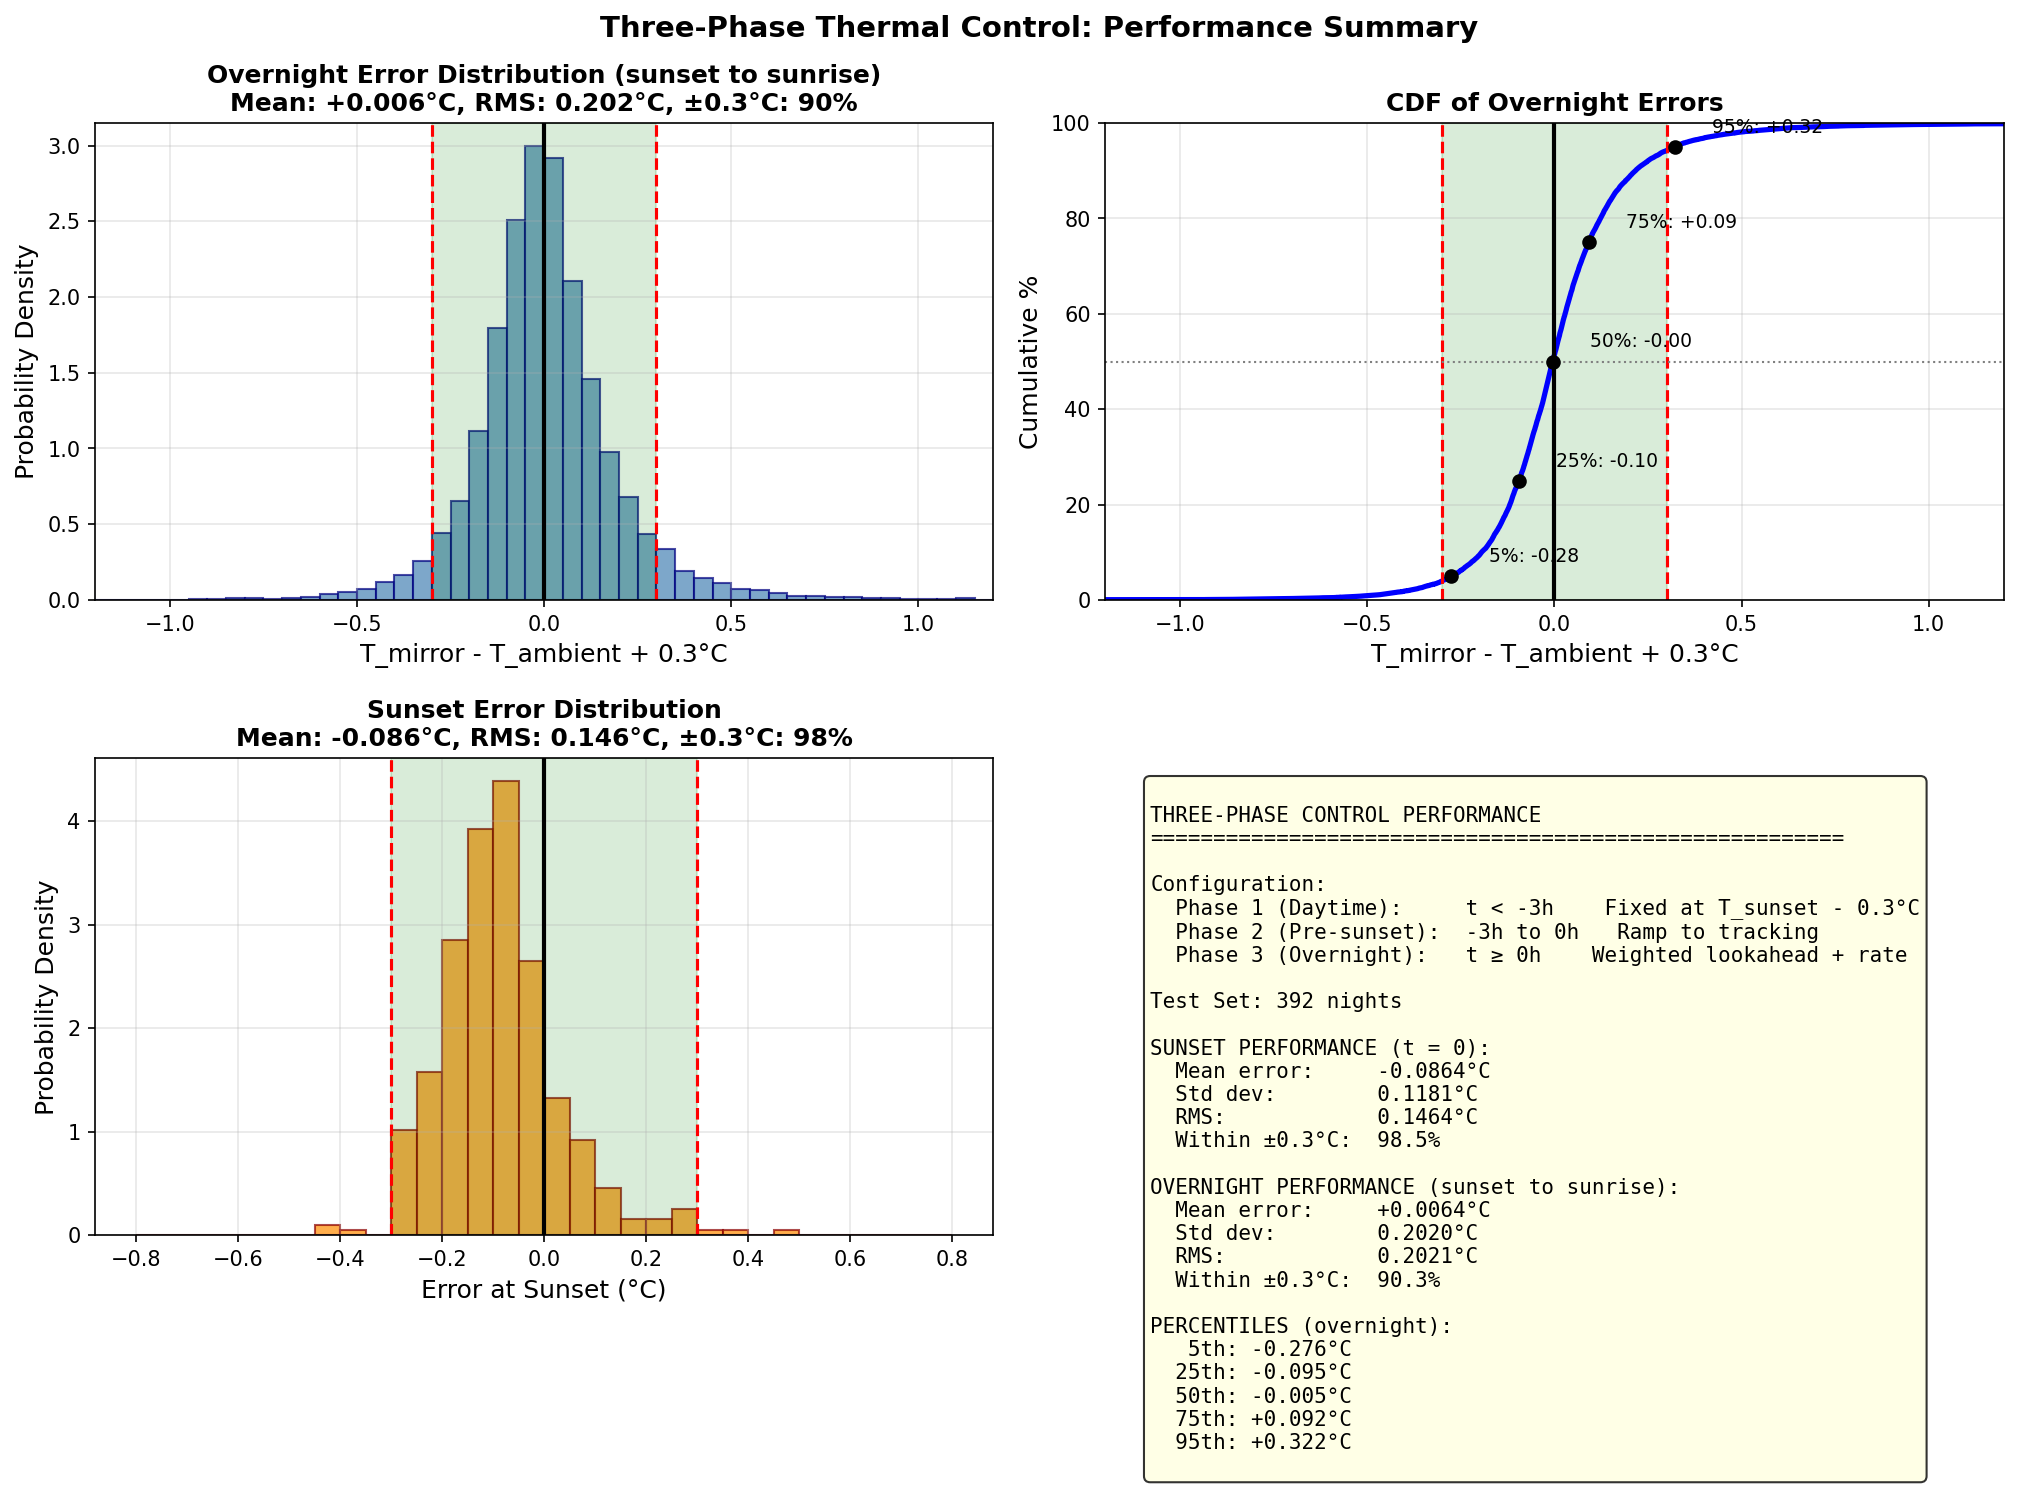
\includegraphics[width=0.95\textwidth]{three_phase_histograms.png}
\caption{RAMP algorithm performance histograms. Top left: overnight error distribution. Top right: cumulative distribution function with percentile markers. Bottom left: sunset error distribution. Bottom right: summary statistics.}
\label{fig:histograms}
\end{figure}

\subsection{Example Night Simulations}

Figure~\ref{fig:examples} shows the algorithm performance across diverse weather conditions.

\begin{figure}[H]
\centering
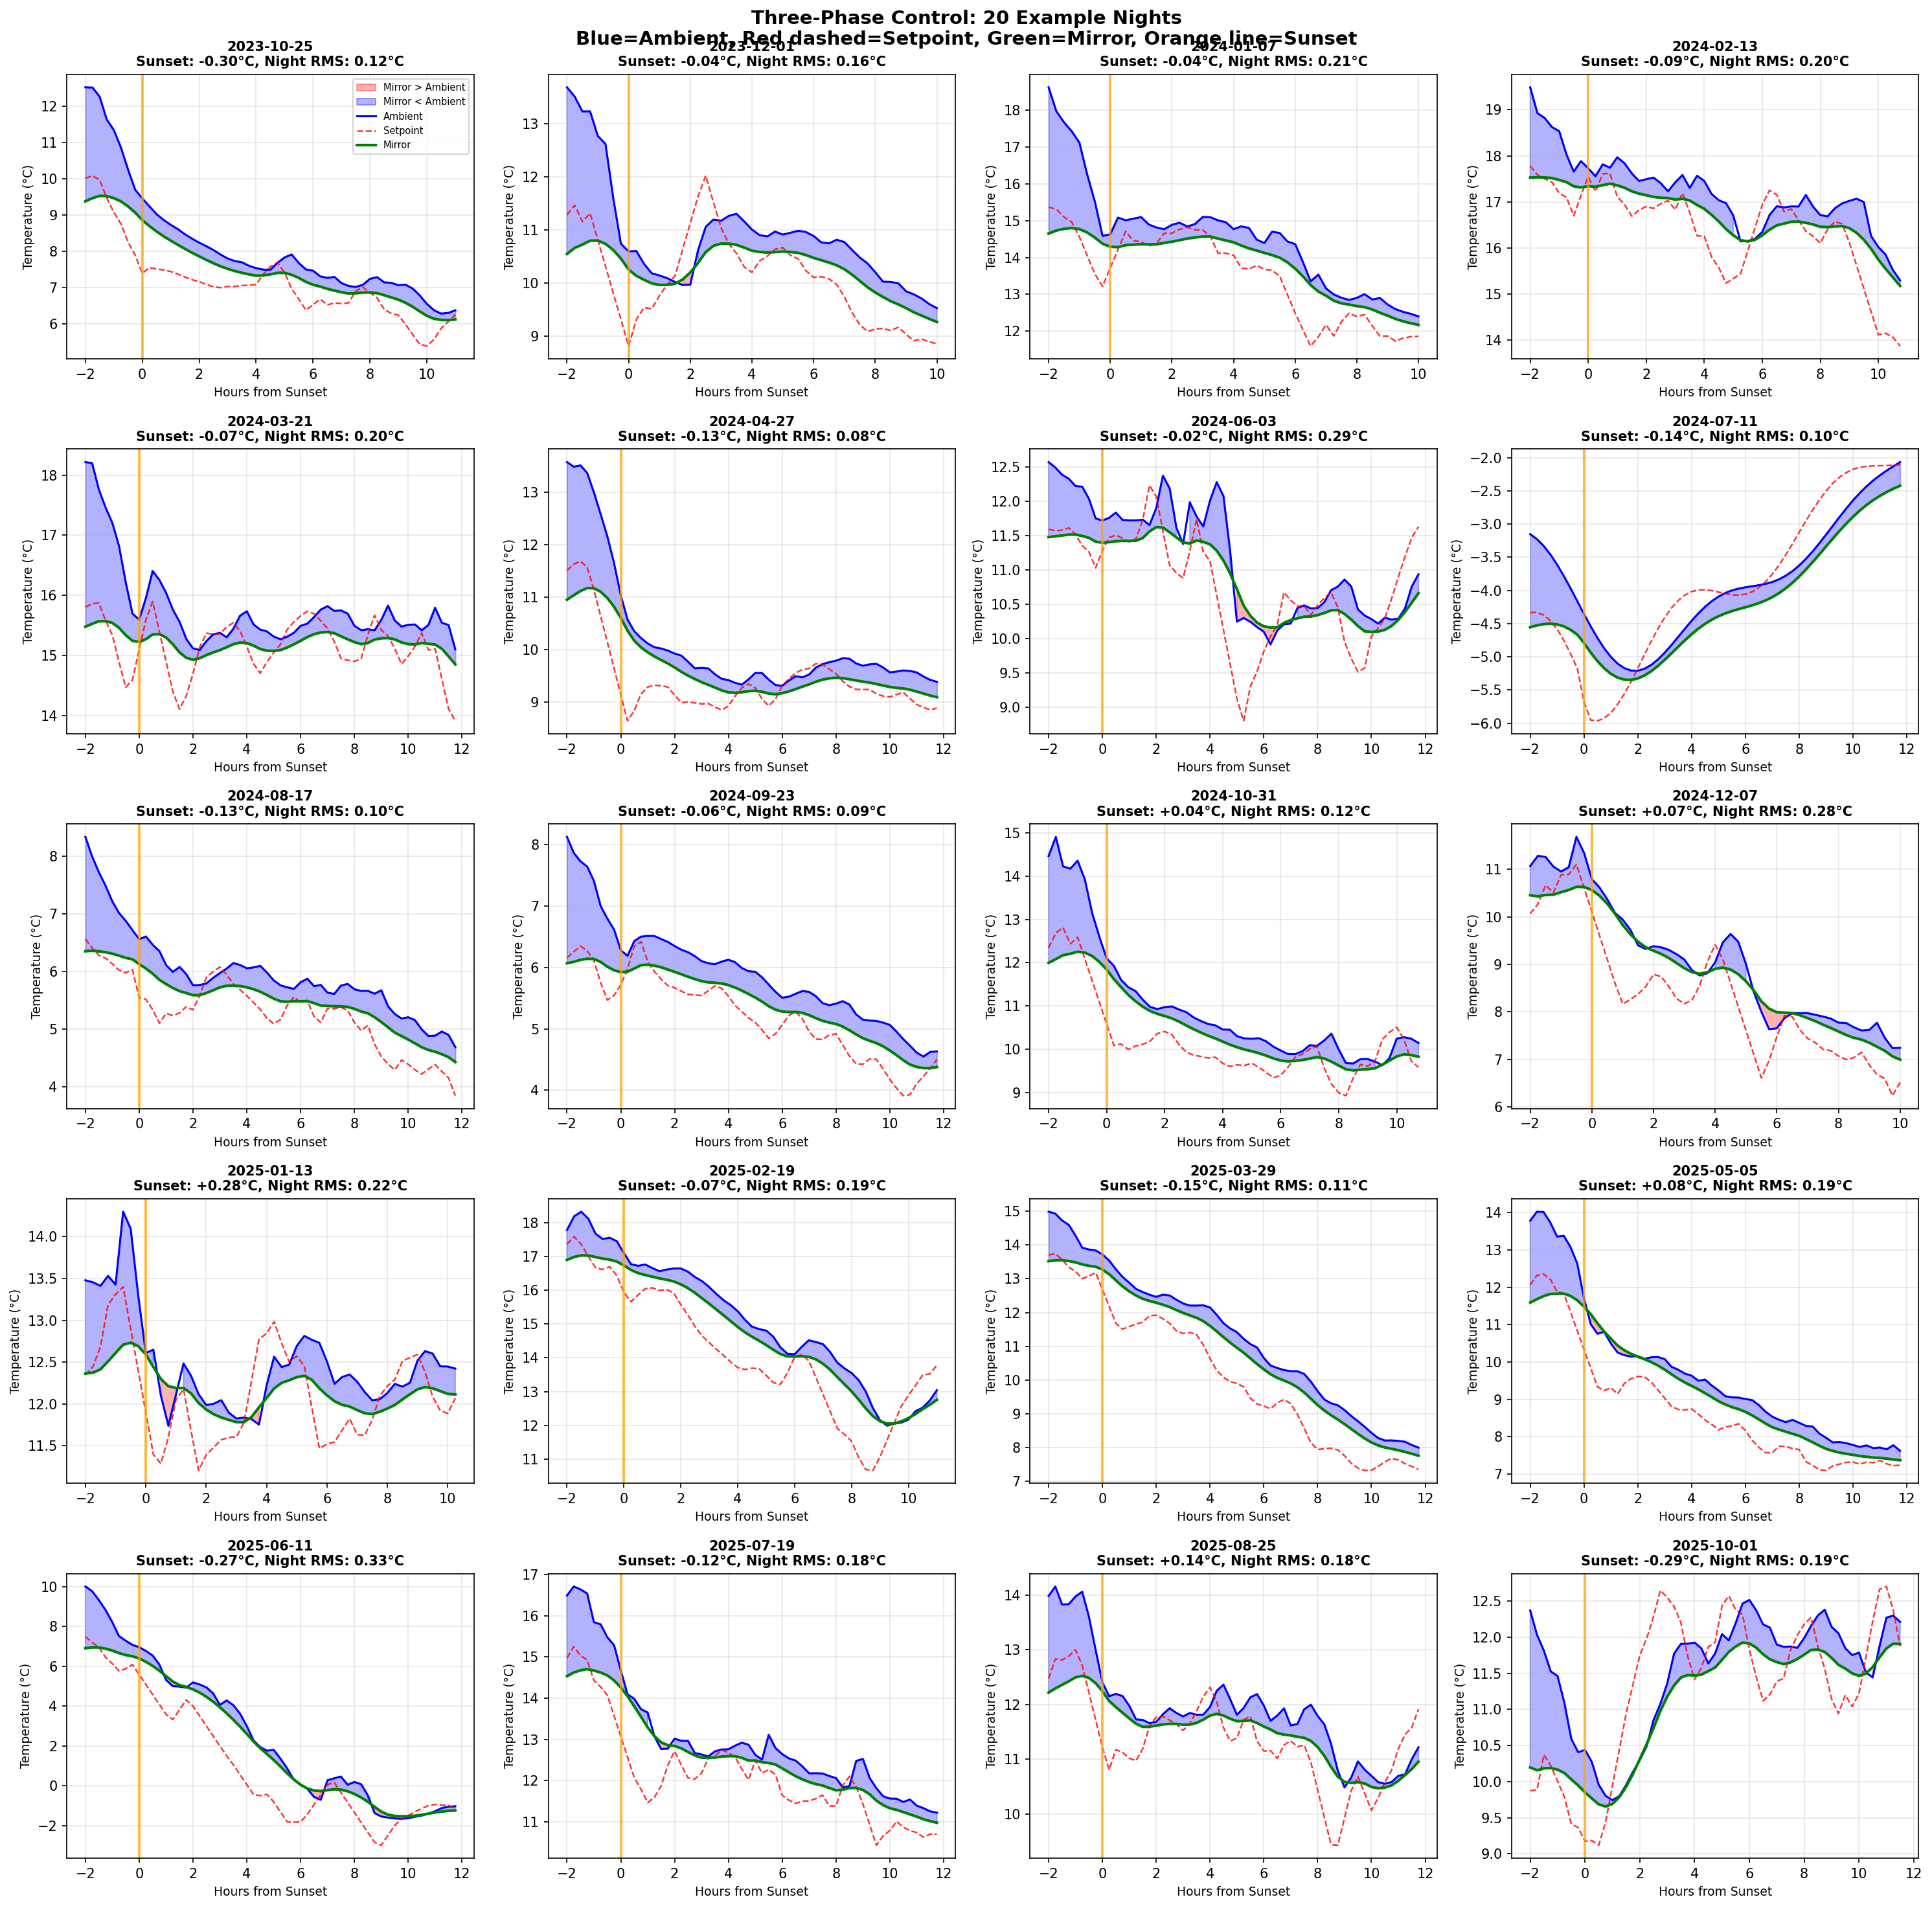
\includegraphics[width=0.95\textwidth]{three_phase_20_nights.png}
\caption{RAMP algorithm performance on 20 example nights from the test set. Blue regions indicate mirror cooler than ambient (desired), red regions indicate mirror warmer than ambient (undesired). Orange vertical line marks sunset.}
\label{fig:examples}
\end{figure}

\subsection{Continuous Three-Day Operation}

Figure~\ref{fig:3day} illustrates the RAMP algorithm operating continuously over three consecutive days, demonstrating the seamless transitions between the three control phases across multiple day-night cycles.

\begin{figure}[H]
\centering

\includegraphics[width=0.98\textwidth]{three_phase_3day.png}
\caption{RAMP algorithm performance over three consecutive days showing continuous operation through multiple day-night cycles. The plot demonstrates the three-phase transitions: daytime fixed setpoint (Phase 1), pre-sunset ramp (Phase 2), and overnight weighted lookahead tracking (Phase 3). Yellow shading indicates daytime periods when the dome is closed.}
\label{fig:3day}
\end{figure}

\subsection{Comparison with Baseline Algorithms}

\begin{table}[H]
\centering
\caption{Algorithm comparison on test set}
\begin{tabular}{lccc}
\toprule
\textbf{Algorithm} & \textbf{RMS ($^\circ$C)} & \textbf{$\pm$0.3$^\circ$C} & \textbf{Improvement} \\
\midrule
Match ambient & 0.63 & 58\% & -- \\
Ambient $-0.75^\circ$C & 0.73 & 49\% & -16\% \\
Single lookahead ($\tau$) & 0.28 & 82\% & 56\% \\
\textbf{RAMP (three-phase)} & \textbf{0.20} & \textbf{90\%} & \textbf{68\%} \\
\bottomrule
\end{tabular}
\end{table}

%==============================================================================
\section{Implementation Considerations}
%==============================================================================

\subsection{Prediction Requirements}

The RAMP algorithm requires temperature predictions with:
\begin{itemize}[noitemsep]
    \item \textbf{Lead time}: 3 hours for overnight lookahead
    \item \textbf{Update frequency}: 15 minutes (matching simulation timestep)
    \item \textbf{Accuracy}: RMS $<$1$^\circ$C at 3-hour lead time (achieved by Random Forest predictor)
\end{itemize}

\subsection{Computational Requirements}

Each setpoint calculation requires:
\begin{itemize}[noitemsep]
    \item 13 temperature lookups (interpolated)
    \item 1 rate calculation (finite difference)
    \item Weighted sum and bias subtraction
\end{itemize}

Computational cost is negligible ($<$1 ms per update).

\subsection{Fallback Modes}

If predictions become unavailable:
\begin{enumerate}[noitemsep]
    \item \textbf{Primary fallback}: Reactive control with rate compensation
    \item \textbf{Secondary fallback}: Naive tracking (current ambient $-$ 0.3$^\circ$C)
\end{enumerate}

%==============================================================================
\section{Conclusions}
%==============================================================================

The RAMP (Rubin Anticipatory Mirror Protocol) algorithm provides effective thermal control for the Rubin Observatory primary mirror through:

\begin{enumerate}
    \item \textbf{Three-phase operation} optimized for the daytime-to-nighttime transition
    \item \textbf{Weighted lookahead prediction} that balances near-term reliability with longer-term anticipation
    \item \textbf{Rate compensation} that accounts for temperature dynamics
    \item \textbf{Smooth transitions} that respect the mirror's thermal time constant
\end{enumerate}

Key performance metrics:
\begin{itemize}[noitemsep]
    \item Overnight RMS error: 0.20$^\circ$C
    \item Time within $\pm$0.3$^\circ$C: 90\%
    \item 68\% improvement over naive control
\end{itemize}

The algorithm is robust across diverse weather conditions and provides consistent performance throughout the observing season.

%==============================================================================
\appendix
\section{Algorithm Pseudocode}
%==============================================================================

\begin{verbatim}
function RAMP_setpoint(t, T_ambient, T_predicted[], T_sunset_predicted):

    # Phase determination
    hours_before_sunset = sunset_time - t

    if hours_before_sunset > 3:
        # Phase 1: Daytime fixed
        return T_sunset_predicted - 0.3

    else if hours_before_sunset > 0:
        # Phase 2: Pre-sunset ramp
        alpha = (3 - hours_before_sunset) / 3
        rate = compute_rate(T_ambient, window=1h)
        T_fixed = T_sunset_predicted - 0.3
        T_track = T_ambient - 0.3 + 0.5 * TAU * rate
        return (1 - alpha) * T_fixed + alpha * T_track

    else:
        # Phase 3: Overnight weighted lookahead
        weights = linear_kernel(n=13, T_max=3h)
        T_weighted = sum(w * T_predicted[t + dt] for w, dt in weights)
        rate = compute_rate(T_ambient, window=1h)
        return T_weighted + 0.5 * TAU * rate - 0.3

    # Apply rate limiting
    setpoint = clip(setpoint, prev_setpoint - 0.5, prev_setpoint + 0.5)
    return setpoint
\end{verbatim}

\end{document}
